\documentclass{article}

\usepackage{arxiv}

\usepackage[utf8]{inputenc} % allow utf-8 input
\usepackage[T1]{fontenc}    % use 8-bit T1 fonts
\usepackage{hyperref}       % hyperlinks
\usepackage{url}            % simple URL typesetting
\usepackage{booktabs}       % professional-quality tables
\usepackage{amsfonts}       % blackboard math symbols
\usepackage{nicefrac}       % compact symbols for 1/2, etc.
\usepackage{microtype}      % microtypography
\usepackage{lipsum}    % 自動產生亂文
\usepackage{graphicx}  % 使用圖片
\usepackage{listings}   % 使用程式碼嵌入
\usepackage{fontspec}   %加這個就可以設定字體
\usepackage{xeCJK}       %讓中英文字體分開設置
\setCJKmainfont{細明體} % SimSun, 標楷體, 設定中文為系統上的字型,而英文不去更動,使用原TeX字型
\XeTeXlinebreaklocale "zh"             %這兩行一定要加,中文才能自動換行
\XeTeXlinebreakskip = 0pt plus 1pt     %這兩行一定要加,中文才能自動換行
\renewcommand{\baselinestretch}{1.5} % 行與行之間的間距加大 1.5 倍


\title{從爬山演算法開始學習人工智慧的優化算法}


\author{
  陳鍾誠\thanks{使用註腳來進一步說明}\\
  金門大學資訊工程系\\
  \texttt{ccc@nqu.edu.tw} \\
  %% examples of more authors
}

\begin{document}
\maketitle

\begin{abstract}
我們使用爬山演算法,結合編譯器技術,創造了一個自動求的符號的解方程式套件 eq6.js,雖然並非所有方程式都能求得符號解,但是對《線性方程組、多項式與常係數微分方程式》而言,通常可以求得正確解答,而對其他更複雜的微分方程或偏微分方程,則無法保證能得到正確解答。
\end{abstract}


% keywords can be removed
\keywords{方程式求解\and 符號微分\and 人工智慧}

\section{簡介}

測是測試!

爬山演算法 (Hill Climbing) 是一種非常簡單的優化算法,該方法模擬人類爬山時的行為,因此稱為爬山演算法。

程式究竟要怎麼爬山呢?且讓我們用一張圖來看看。假如我們在 Google 裏輸入一個算式,Google 會幫我們畫出該函數。舉例而言,如果我在 Google 輸入 $x^2+3x+5$  這個算式,您會看到如圖 \ref{fig:curve1} 所示的結果。

\begin{figure}
  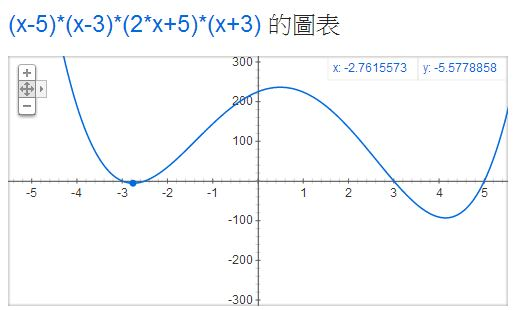
\includegraphics[width=\linewidth]{img/GoogleGraph2Dvally.jpg}
  \caption{在 Google 輸入 $x^2+3x+5$ 後顯示的函數圖}
  \label{fig:curve1}
\end{figure}


這時您可以移動滑鼠,圖形會出現一個可移動的小藍點,該點會沿著曲線移動,上圖中 (x, y) 座標顯示為 x:6.07202181, y:60.0855143,
就是那個小藍點所在的位置。如果我們想要寫程式尋找這個函數的最低點,那我們應該怎麼找呢?

其實方法很簡單,就是一直往低的地方走,一直走到最低點,然後你會看到左右兩邊都沒辦法更低了,於是就停止尋找,傳回該最低點作為答案。這個方法,就像是水往低處流一樣,不斷的往更低的方向流,最後一定會流到一個山谷,然後就積成一個湖了。

但是、既然這樣,那為甚麼叫做爬山演算法,而不叫「流水下山演算法」呢?其 實、只要反過來看就行了,如果我們想要找的是最高點,而不是最低點,那整個行為就會像爬山一樣,只是最後爬到山頂就會停了。採用這種想法,若我們想找 $x^2+3x+5$ 這個函數的最高,我們可以在 Google 輸入  $-(x^2+3x+5)$  就可以看到那座山了,圖  \ref{fig:curve2} 是 Google 顯示的結果  :

\begin{figure}
  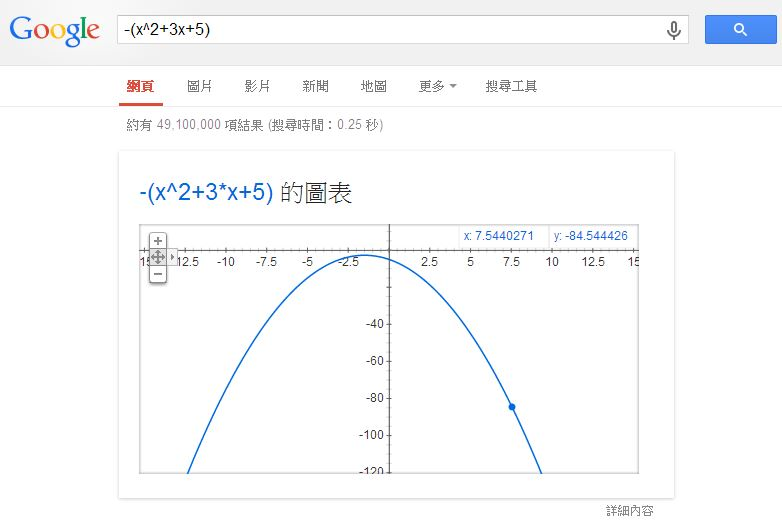
\includegraphics[width=\linewidth]{img/GoogleGraph2DMountain.jpg}
  \caption{在 Google 輸入 $-(x^2+3x+5)$ 後顯示的函數圖}
  \label{fig:curve2}
\end{figure}

\section{方法}


假如我們在上圖中左邊的山谷,那麼怎麼能知道右邊還有一個更低的山谷呢?這就是「流水下山演算法」的困難之所在了!

當然、也有人試圖提出一些企圖找到更深的谷,或爬到更高的山的演算法,這些演算法往往是以爬山演算法為基礎,然後再作一些改良,像是「模擬退火演算法」(Simulated Annealing Algorithm) 或大洪水演算法 (Great Deluge algorithm) 等等,這些方法都是企圖讓「流水下山演算法」有機會跳出山谷而設計的方法。

當然、您也可以企圖加上「衝力」之類的想法讓「流水下山演算法」可以衝出低谷,但是到底要衝多久,還有該往哪個方向衝才對呢?那這種方法是否該改叫「衝山演算法」呢?

當然、我是沒有聽過這種名稱啦!

另外、對於上述的單變數函數而言,不是往左邊走就是往右邊走,但是如果有兩個變數,例如像  $x^2+y^2+3x+5y+6$  ,但是只有一個山谷,那麼我們該修改哪個變數呢?舉例而言,以下就是 Google 所畫出的  $x^2+y^2+3x+5y+6$  之圖形  \ref{fig:curve3} 。

\begin{figure}
  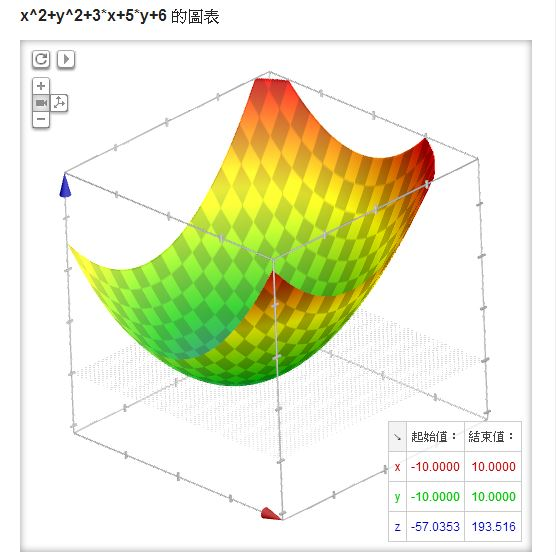
\includegraphics[width=\linewidth]{img/GoogleGraph3D.jpg}
  \caption{Google 所畫出的 $x^2+y^2+3x+5y+6$  之圖形}
  \label{fig:curve3}
\end{figure}



在上述的雙變數情形中,我們可以隨機的挑一個變數,然後向左或向右移動一小步,只要移動後的點更低就接受,如果連續很多次移動都沒辦法找到更低的點,就認為已經到達山谷,這樣的方法其實還蠻有效的,這種方法可以稱為「隨機下山演算法」 (反過來英文中以爬山的角度來看,所以稱為隨機爬山演算法 Stochastic Hill Climbing Algorithm)。
在上圖中,底下的平面上所畫的向量,就是上面那個曲面在該點的梯度,換句話說某一點的梯度其實是一個向量。梯度的計算公式如下:


\begin{equation}
\nabla f  = \frac{\partial f}{\partial x_1 }\vec{e_1} + \cdots + \frac{\partial f}{\partial x_n }\vec{e_n}
\end{equation}


如果我們可以計算某函數之梯度的話,那麼就可以不用透過隨機的方式去亂走了,只要朝著梯度的方向走去,就是最快下降的道路了。

如果我們採用這種沿著梯度方向往下走的方法,就稱為「梯度下降法」(Gradient Descent),這種方法可以說是一種「貪婪演算法」(Greedy Algorithm),因為它每次都朝著最斜的方向走去,企圖得到最大的下降幅度。

在「神經網路」中的「反傳遞演算法」,其實就是一種梯度下降法,所以才會有下列這段程式:

\begin{lstlisting}
function sigmoid(x) {
  return ml.tanh(x);
}

function dsigmoid(y) {
  return 1.0 - y*y;
}
\end{lstlisting}


其中的 sigmoid(x) 設定為 tanh(x) 這個函數,tanh(x) 的數學定義如下:

\begin{equation}
\sinh x = {{e^x  - e^{ - x} } \over 2} \\
\cosh x = {{e^x  + e^{ - x} } \over 2} \\
\tanh x = {{\sinh x} \over {\cosh x}}\\
\end{equation}

而 dsigmoid(y) 中的  1.0 - y*y  則是 y=tanh(x) 的微分式,對每個 y=tanh(x) 都取微分式的時候,其實就是梯度的方向,因此「反傳遞演算法」事實上是一種梯度下降法啊!

這時,或許各位會想起,「貪婪演算法」怎麼感覺有點熟悉,似乎在哪裡學過?

如果各位學過演算法課程,或許想起像「最小擴展樹」(Minimal Spanning Tree) 的演算法,您會想到這種方法也很貪婪,因為每次都找最小的邊來加入,那也是一種「貪婪演算法」,但這與此處的貪婪演算法之概念顯然有些差距了。



\bibliographystyle{unsrt}  
%\bibliography{references}  %%% Remove comment to use the external .bib file (using bibtex).
%%% and comment out the ``thebibliography'' section.


%%% Comment out this section when you \bibliography{references} is enabled.
\begin{thebibliography}{1}

\bibitem{}
陳鍾誠
\newblock 爬山演算法
\newblock (2017) github pages, e103.

\bibitem{10.7717/peerj-cs.103}
Meurer, Aaron and Smith, Christopher P. and Paprocki, Mateusz
\newblock SymPy: symbolic computing in Python,
\newblock (2017) SymPy: symbolic computing in Python. PeerJ Computer Science 3:e103.

\bibitem{kour2014real}
George Kour and Raid Saabne.
\newblock Real-time segmentation of on-line handwritten arabic script.
\newblock In {\em Frontiers in Handwriting Recognition (ICFHR), 2014 14th
  International Conference on}, pages 417--422. IEEE, 2014.

\bibitem{kour2014fast}
George Kour and Raid Saabne.
\newblock Fast classification of handwritten on-line arabic characters.
\newblock In {\em Soft Computing and Pattern Recognition (SoCPaR), 2014 6th
  International Conference of}, pages 312--318. IEEE, 2014.

\bibitem{hadash2018estimate}
Guy Hadash, Einat Kermany, Boaz Carmeli, Ofer Lavi, George Kour, and Alon
  Jacovi.
\newblock Estimate and replace: A novel approach to integrating deep neural
  networks with existing applications.
\newblock {\em arXiv preprint arXiv:1804.09028}, 2018.

\end{thebibliography}


\end{document}
